% Created 2024-09-10 Tue 21:08
% Intended LaTeX compiler: xelatex
\documentclass[11pt]{article}
\usepackage{graphicx}
\usepackage{longtable}
\usepackage{wrapfig}
\usepackage{rotating}
\usepackage[normalem]{ulem}
\usepackage{capt-of}
\usepackage{hyperref}
\usepackage{minted}
\usepackage[a4paper, margin=2.5cm]{geometry}
\usepackage{minted}
\usepackage{fontspec}
\setmonofont{Iosevka}
\setminted{fontsize=\small, frame=single, breaklines=true}
\usemintedstyle{emacs}
\usepackage[backend=biber,style=apa]{biblatex}
\addbibresource{citation.bib}
\usepackage{amsmath}
\allowdisplaybreaks
\author{Baley Eccles - 652137}
\date{\textit{{[}2024-09-03 Tue 17:10]}}
\title{kme272 - Assesment 1.5}
\hypersetup{
 pdfauthor={Baley Eccles - 652137},
 pdftitle={kme272 - Assesment 1.5},
 pdfkeywords={},
 pdfsubject={},
 pdfcreator={Emacs 29.4 (Org mode 9.8)}, 
 pdflang={English}}
\begin{document}

\maketitle
\tableofcontents

\section{kme272 - Assesment 1.5}
\label{sec:orge4f22a3}
\subsection{Q1}
\label{sec:org3bab8c5}


\begin{minted}[]{octave}
clear
clc
pkg load symbolic
x_0=-4;
x_1=0;
x_2=4;
y_0=3;
y_1=5;
y_2=1;
syms x L_1 L_2 L_3


L_0 = ((x - x_1) * (x - x_2)) / ((x_0 - x_1) * (x_0 - x_2));
L_1 = ((x - x_0) * (x - x_2)) / ((x_1 - x_0) * (x_1 - x_2));
L_2 = ((x - x_0) * (x - x_1)) / ((x_2 - x_0) * (x_2 - x_1));
% Display the LaTeX representations
latex(L_0)
latex(L_1)
latex(L_2)
P_2=y_0*L_0+y_1*L_1+y_2*L_2;
latex(P_2)
\end{minted}


\[L_0(x)=\frac{(x - x_1) \cdot (x - x_2)}{{}(x_0 - x_1) \cdot (x_0 - x_2)}=\frac{x \left(x - 4\right)}{32}\]
\[L_1(x)=\frac{(x - x_0) \cdot (x - x_2)}{{}(x_1 - x_0) \cdot (x_1 - x_2)}=-\frac{\left(x - 4\right) \left(x + 4\right)}{16}\]
\[L_2(x)=\frac{(x - x_0) \cdot (x - x_1)}{{}(x_2 - x_0) \cdot (x_2 - x_1)}=\frac{x \left(x + 4\right)}{32}\]
\[P_2(x)=y_0\cdot L_0(x) + y_1\cdot L_1(x) + y_2\cdot L_2(x) = \frac{3 x \left(x - 4\right)}{32} + \frac{x \left(x + 4\right)}{32} - \frac{5 \left(x - 4\right) \left(x + 4\right)}{16}\]
\subsection{Q2}
\label{sec:org55bfbbf}
\begin{itemize}
\item \[f[x_0,x_1]=\frac{y_1-y_0}{x_1-x_0}\]
\item \[f[x_1,x_2]=\frac{y_2-y_1}{x_2-x_1}\]
\item \[f[x_2,x_3]=\frac{y_3-y_2}{x_3-x_2}\]
\item \[f[x_0,x_1,x_2]=\frac{y_1-y_0}{x_1-x_0}-\frac{y_2-y_1}{x_2-x_1}\]
\item \[f[x_1,x_2,x_3]=\frac{y_2-y_1}{x_2-x_1}-\frac{y_3-y_2}{x_3-x_2}\]
\item \[f[x_0,x_1,x_2,x_3]=\frac{f[x_1,x_2,x_3]-f[x_0,x_1,x_2]}{x_3-x_0}\]
\end{itemize}
Using these equations we can fill in the table \\
\begin{tabular}{|c|c|c|c|c|}
x & f[x] & f[x_0,x_1] & [f[x_0,x_1,x_2] & f[x_0,x_1,x_2,x_3] \\
-4 & 3 &  &  & \\
0 & 5 & 0.5 &  & \\
4 & 1 & -1 & -0.1875 & \\
6 & -1 & -1 & 0 & 0.01875 \\
\end{tabular}


\[P_3(x)=f[x_0​]+f[x_0​,x_1​](x - x_0​)+f[x_0​,x_1​,x_2​](x - x_0​)(x - x_1​)+f[x_0​,x_1​,x_2​,x_3​](x - x_0​)(x - x_1​)(x - x_2​)\]
\[P_3(x)=3+0.5(x+4)-1(x+4)(x)-0.01875(x+4)(x)(x-4)\]
\subsection{Q3}
\label{sec:org5994f63}

\begin{minted}[]{octave}
clear
clc
pkg load symbolic
syms Mn hn xn1 Mn1 hn yn yn1 xn a hn1
sn=(Mn1/(6*hn1))*(xn-xn)^3 +(Mn/(6*hn1))*(xn-xn1)^3 + ((yn1/hn1)-(1/6)*hn1*Mn1)*(xn-xn)+((yn/hn1)-(1/6)*hn1*Mn)*(xn-xn1);
snDiff=(-Mn1/(2*hn1))*(xn-xn)^2+(Mn/(2*hn1))*(xn-xn1)^2+(hn1/6)*(Mn1-Mn)+((yn-yn1)/hn1);
eq= sn+snDiff == a;
latex(eq)
\end{minted}

\[\frac{M_n \left(x_n - x_{n-1}\right)^{3}}{6 h_{n-1}} + \frac{M_n \left(x_n - x_{n-1}\right)^{2}}{2 h_{n-1}} + \frac{h_{n-1} \left(- M_n + M_{n-1}\right)}{6}\]
\[+\left(x_n - x_{n-1}\right) \left(- \frac{M_n h_{n-1}}{6} + \frac{y_n}{h_{n-1}}\right) + \frac{y_n - y_{n-1}}{h_{n-1}} = \alpha\]
\subsection{Q4}
\label{sec:org29f37e3}
\begin{minted}[]{octave}
clear
clc
pkg load symbolic
syms M0 M1 M2 h0 h1 h2 x0 x1 x2 y0 y1 y2 a x
s0=(M0/(6*h0))*(x1-x1)^3 +(M1/(6*h0))*(x1-x)^3 + ((y0/h0)-(0/6)*h0*M0)*(x1-x1)+((y1/h0)-(0/6)*h0*M1)*(x1-x);
eq1=subs(diff(diff(s0,x),x),x,x0);
latex(expand(simplify(eq1)))


s1=(M1/(6*h1))*(x2-x2)^3 +(M2/(6*h1))*(x2-x1)^3 + ((y1/h1)-(1/6)*h1*M1)*(x2-x2)+((y2/h1)-(1/6)*h1*M2)*(x2-x1);
eq2= s1+diff(s1,x2)==a;
latex(expand(simplify(eq2)))

\end{minted}

Which gives the two following equations:
\[-\frac{M_{1} x_{0}}{h_{0}} + \frac{M_{1} x_{1}}{h_{0}}=0\]

\[a = \frac{M_{2} h_{1} x_{1}}{6} - \frac{M_{2} h_{1} x_{2}}{6} - \frac{M_{2} h_{1}}{6} - \frac{M_{2} x_{1}^{3}}{6 h_{1}} + \frac{M_{2} x_{1}^{2} x_{2}}{2 h_{1}} + \frac{M_{2} x_{1}^{2}}{2 h_{1}} - \frac{M_{2} x_{1} x_{2}^{2}}{2 h_{1}} - \frac{M_{2} x_{1} x_{2}}{h_{1}} + \frac{M_{2} x_{2}^{3}}{6 h_{1}} + \frac{M_{2} x_{2}^{2}}{2 h_{1}}\]
\[-\frac{x_{1} y_{2}}{h_{1}} + \frac{x_{2} y_{2}}{h_{1}} + \frac{y_{2}}{h_{1}}\]


And in matrix form:
\[\begin{bmatrix}
-\frac{x_{0}}{h_{0}} + \frac{x_{1}}{h_{0}} & 0 \\
0 & \frac{M_{2} h_{1} x_{1}}{6} -\frac{M_{2} h_{1} x_{2}}{6}+\frac{M_{2} h_{1}}{6}- \frac{M_{2} x_{1}^{3}}{6 h_{1}} + \frac{M_{2} x_{1}^{2} x_{2}}{2 h_{1}} - \frac{M_{2} x_{1}^{2}}{2 h_{1}} - \frac{M_{2} x_{1} x_{2}^{2}}{2 h_{1}} + \frac{M_{2} x_{1} x_{2}}{h_{1}} + \frac{M_{2} x_{2}^{3}}{6 h_{1}} - \frac{M_{2} x_{2}^{2}}{2 h_{1}}
\end{bmatrix} \begin{bmatrix}
M_1 \\
M_2
\end{bmatrix}\]
\[= \begin{bmatrix}
0 \\
\alpha + \frac{x_{1} y_{2}}{h_{1}} - \frac{x_{2} y_{2}}{h_{1}} + \frac{y_{2}}{h_{1}}\]
\end{bmatrix}$\backslash$]
\subsection{Q5}
\label{sec:orgc3d21d3}

\begin{minted}[]{octave}
clear
clc
pkg load symbolic
syms M0 M1 M2 h0 h1 h2 x0 x1 x2 y0 y1 y2 a x x3 y3
s0=(M0/(6*h0))*(x1-x1)^3 +(M1/(6*h0))*(x1-x)^3 + ((y0/h0)-(0/6)*h0*M0)*(x1-x1)+((y1/h0)-(0/6)*h0*M1)*(x1-x);
eq1=subs(diff(diff(s0,x),x),x,x0);
s1=(M1/(6*h1))*(x2-x2)^3 +(M2/(6*h1))*(x2-x1)^3 + ((y1/h1)-(1/6)*h1*M1)*(x2-x2)+((y2/h1)-(1/6)*h1*M2)*(x2-x1);
eq2= s1+diff(s1,x2)==a;

x0value=-4;
x1value=0;
x2value=4;
x3value=6;
y0value=3;
y1value=5;
y2value=1;
y3value=-1;
h0value=x1value-x0value;
h1value=x2value-x1value;
h2value=x3value-x2value;
avalue=1/2;

eq1=subs(eq1,x0,x0value);
eq1=subs(eq1,x1,x1value);
eq1=subs(eq1,x2,x2value);
eq1=subs(eq1,x3,x3value);
eq1=subs(eq1,y0,y0value);
eq1=subs(eq1,y1,y1value);
eq1=subs(eq1,y2,y2value);
eq1=subs(eq1,y3,y3value);
eq1=subs(eq1,h0,h0value);
eq1=subs(eq1,h1,h1value);
eq1=subs(eq1,h2,h2value);
eq1=subs(eq1,a,avalue);

eq2=subs(eq2,x0,x0value);
eq2=subs(eq2,x1,x1value);
eq2=subs(eq2,x2,x2value);
eq2=subs(eq2,x3,x3value);
eq2=subs(eq2,y0,y0value);
eq2=subs(eq2,y1,y1value);
eq2=subs(eq2,y2,y2value);
eq2=subs(eq2,y3,y3value);
eq2=subs(eq2,h0,h0value);
eq2=subs(eq2,h1,h1value);
eq2=subs(eq2,h2,h2value);
eq2=subs(eq2,a,avalue);

latex(expand(simplify(eq1)))
latex(expand(simplify(eq2)))

\end{minted}
Subsituting the values into the two equations gives:
\[M_{1}=0\]
\[M_{2} = - \frac{9}{16}\]
Which gives the matrix equation:
\[\begin{bmatrix}
1 & 0 \\
0 & 1\\
\end{bmatrix} \begin{bmatrix}
M_1 \\
M_2
\end{bmatrix} = \begin{bmatrix}
0 \\
-\frac{9}{16}
\end{bmatrix}\]
\subsection{Q6}
\label{sec:org8065d2a}

\begin{minted}[]{octave}
% Given data points
x = [-4, 0, 4, 6];
y = [3, 5, 1, -1];
alpha = -1/2;

% Construct the matrix for the spline
A = [1, 0; 0, 1];
b = [0; alpha];

% Solve for M1 and M2
M = A\b;

% Generate spline
xx = linspace(-4, 6, 100);
yy = spline(x, [M(1), y, M(2)], xx);

% Plotting
figure;
plot(xx, yy, 'r-', 'LineWidth', 2);
hold on;

% Overlay the Lagrange polynomial
P2 = @(x) ... % Define P2 based on your calculations
plot(xx, P2(xx), 'b--', 'LineWidth', 2);
legend('Cubic Spline', 'Lagrange Polynomial');
title('Cubic Spline and Lagrange Polynomial');
xlabel('x');
ylabel('y');
grid on;
hold off;
filename = sprintf('KME272-Assignment-5.png');
print(filename,'-dpng','-r100');
\end{minted}

\begin{center}
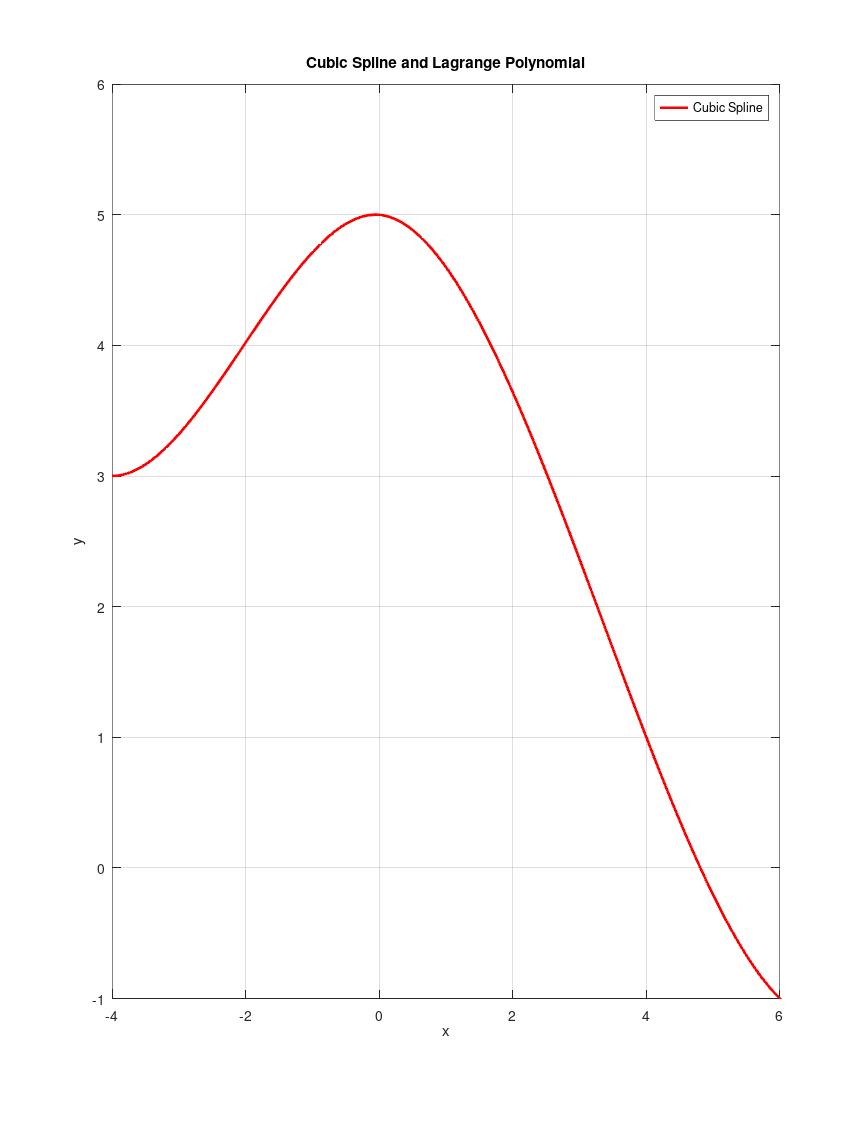
\includegraphics[width=.9\linewidth]{KME272-Assignment-5.png}
\end{center}
\end{document}
